%\documentclass[12pt]{article}
\documentclass[12pt]{scrartcl}
\title{Assignment Template}
\nonstopmode
%\usepackage[utf-8]{inputenc}
\usepackage{lipsum}
\usepackage{graphicx} % Required for including pictures
\usepackage[figurename=Figure]{caption}
\usepackage{float}    % For tables and other floats
\usepackage{verbatim} % For comments and other
\usepackage{amsmath}  % For math
\usepackage{amssymb}  % For more math
\usepackage{fullpage} % Set margins and place page numbers at bottom center
\usepackage{paralist} % paragraph spacing
\usepackage{listings} % For source code
\usepackage{subfig}   % For subfigures
%\usepackage{physics}  % for simplified dv, and 
\usepackage{enumitem} % useful for itemization
\usepackage{siunitx}  % standardization of si units

\usepackage{tikz,bm} % Useful for drawing plots
%\usepackage{tikz-3dplot}
\usepackage{circuitikz}

%%% Colours used in field vectors and propagation direction
\definecolor{mycolor}{rgb}{1,0.2,0.3}
\definecolor{brightgreen}{rgb}{0.4, 1.0, 0.0}
\definecolor{britishracinggreen}{rgb}{0.0, 0.26, 0.15}
\definecolor{cadmiumgreen}{rgb}{0.0, 0.42, 0.24}
\definecolor{ceruleanblue}{rgb}{0.16, 0.32, 0.75}
\definecolor{darkelectricblue}{rgb}{0.33, 0.41, 0.47}
\definecolor{darkpowderblue}{rgb}{0.0, 0.2, 0.6}
\definecolor{darktangerine}{rgb}{1.0, 0.66, 0.07}
\definecolor{emerald}{rgb}{0.31, 0.78, 0.47}
\definecolor{palatinatepurple}{rgb}{0.41, 0.16, 0.38}
\definecolor{pastelviolet}{rgb}{0.8, 0.6, 0.79}

\lstset{
  basicstyle=\ttfamily\small,
  breaklines=true,
  keywordstyle=\color{ceruleanblue},
  stringstyle=\color{emerald},
  showstringspaces=false
}

\begin{document}

\noindent
\begin{minipage}{0.15\textwidth}
    
\includegraphics[width=\linewidth]{logo_black.png}
\end{minipage}%
\hfill
\begin{minipage}{0.8\textwidth}
    \begin{center}
        {\textbf{\Large Indian Institute of Technology Kanpur}} \\ \vspace{5pt}
        {\textbf{CGS698C --- Bayesian Models \& Data Analysis}}
    \end{center}
\end{minipage}

\vspace{0.4cm}
\hrule
\vspace{0.4cm}
{\hspace{-11.5pt}\textbf{Name:}\ Anandan Iyer \hspace{\fill} \textbf{Due Date:} \today\\
{\textbf{Roll Number:}}\ 240117 \hspace{\fill} \textbf{Assignment:} 05\\
{\textbf{Department:}}\ Mechanical Engineering \\
\hrule

\paragraph*{Part 1:} \textbf{A simple linear regression: Power posing and testosterone}\\
\textbf{Solution: } \\
We estimate the effect of assigning a subject a high power pose versus a low power pose on the change in their testosterone levels. A linear model is fitted using the \texttt{brms} package with weakly informative priors.

\begin{lstlisting}[language=R]
library(brms)

power_pose_dataset <- read.table("df_powerpose.csv", header=T, sep=",")
power_pose_dataset$testosterone_change <- power_pose_dataset$testm2 - power_pose_dataset$testm1

weakly_informative_priors <- c(
  prior(normal(0, 50), class=Intercept),
  prior(normal(0, 50), class=b)
)

testosterone_regression_model <- brm(
  testosterone_change ~ hptreat, 
  data=power_pose_dataset, 
  prior=weakly_informative_priors, 
  cores=4
)

summary(testosterone_regression_model)
\end{lstlisting}
% The figure environment handles the placement and captioning
\begin{figure}[htbp]
    \centering 
    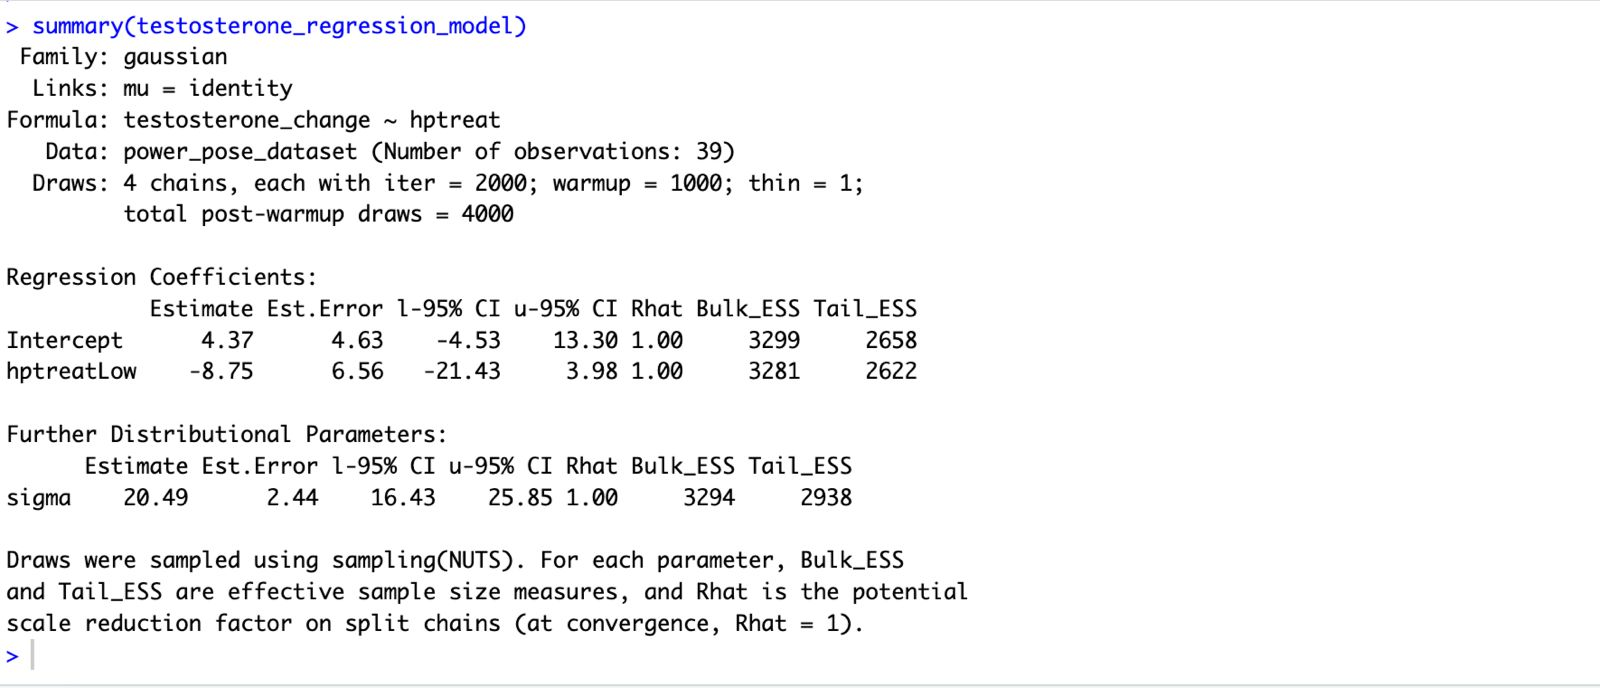
\includegraphics[width=0.9\textwidth]{Figure_1.jpeg}
    \caption{O/P of the above R script}
    \label{fig:my_custom_label}
\end{figure}

\begin{figure}[htbp]
    \centering 
    
\includegraphics[width=0.9\textwidth]{Figure_3.png}
    \caption{Fit Pose}
    \label{fig:my_custom_label}
\end{figure}

\vspace{12pt}
\textbf{b\_hptreatHigh} is the estimated difference in testosterone change between High and Low pose groups. $P(b > 0)$is the posterior probability that high posing increases testosterone relative to low posing.

\newpage
\paragraph*{Part 2:} Poisson regression models and hypothesis testing \\ \\
\textbf{Exercise 2.1} \textbf{Implement the model in R or Python such that the function gives the number of crossings as
the outcome, and takes sentence length, $\alpha$, and $\beta$ as its arguments.} \\ \\
\textbf{Solution: }
\begin{lstlisting}[language=R]
calculate_crossing_dependencies <- function(sentence_length_value, alpha_parameter, beta_parameter) {
  expected_crossing_rate <- exp(alpha_parameter + beta_parameter * sentence_length_value)
  return(rpois(1, expected_crossing_rate))
}
\end{lstlisting} 
\vspace{12pt}
\textbf{Exercise 2.2} \textbf{Generate prior predictions of the model for sentences of length 4 under the following prior assumptions.} \\ 
$\alpha \sim \text{Normal}_{lb=0}(0.15,0.1)$ \\
$\beta \sim \text{Normal}_{lb=0}(0.25,0.05)$ \\
\newline
\textbf{Solution: }
\begin{lstlisting}[language=R]
library(truncnorm)
library(ggplot2)

set.seed(123)
N <- 10000

sample_truncnorm <- function(n, mu, sigma) {
  s <- rnorm(n * 5, mu, sigma)
  s[s >= 0][1:n]
}

alpha_draws <- sample_truncnorm(N, 0.15, 0.1)
beta_draws  <- sample_truncnorm(N, 0.25, 0.05)

prior_pred <- rpois(N, lambda = exp(alpha_draws + beta_draws * 4))
summary(prior_pred)

ggplot(data.frame(x = prior_pred), aes(x = x)) +
  geom_bar(fill = "steelblue") +
  labs(title = "Prior predictive — sentence length 4",
       x = "Number of crossings", y = "Count") +
  theme_classic()
\end{lstlisting}

\begin{figure}[htbp]
    \centering 
    
\includegraphics[width=0.9\textwidth]{Figure_2.png}
    \caption{Prior Predictive}
    \label{fig:my_custom_label}
\end{figure}
\newpage 
\textbf{Exercise 2.3} \textbf{Consider a dataset of crossing dependencies from English and German corpora, "crossing.csv".
This dataset contains number of crossings for each sentence from each language. Fit the following two mod-
els, $M_1$ and $M_2$, to the given data.}
\newline
\textbf{Solution: }
\begin{lstlisting}[language=R]
observed <- read.table("crossings.csv", sep=",", header=T)

observed 
  group_by(Language, s.length) 
  summarise(mean.crossings = mean(nCross), .groups = "drop") 
  ggplot(aes(x = s.length, y = mean.crossings, group = Language, color = Language)) +
  geom_point() + geom_line() +
  theme_classic()

  observed$s.length<-observed$s.length - mean(observed$s.length)
observed$lang<- ifelse(observed$Language == "German", 1, 0)

fit_m1 <- brm(
  nCross ~ 1 + s.length,
  data   = observed,
  family = poisson(link = "log"),
  prior  = c(
    prior(normal(0.15, 0.1), class = Intercept),
    prior(normal(0, 0.15),   class = b)
  ),
  chains = 4, iter = 2000, warmup = 1000, cores = 4, seed = 42
)
summary(fit_m1)

fit_m2 <- brm(
  nCross ~ 1 + s.length + lang + s.length:lang,
  data   = observed,
  family = poisson(link = "log"),
  prior  = c(
    prior(normal(0.15, 0.1), class = Intercept),
    prior(normal(0, 0.15),   class = b)
  ),
  chains = 4, iter = 2000, warmup = 1000, cores = 4, seed = 42
)
summary(fit_m2)
\end{lstlisting}
\newpage
\textbf{Exercise 2.4} \textbf{Quantify evidence for the models $M_1$ and $M_2$ using k-fold cross-validation.}
\newline
\textbf{Solution: }
\begin{lstlisting}[language=R]

set.seed(42)

lpds_m1  <- c()
lpds_m2  <- c()
untested <- observed

for (k in 1:5) {
  ytest    <- sample_n(untested, size = nrow(observed) / 5)
  ytrain   <- setdiff(observed, ytest)
  untested <- setdiff(untested, ytest)

  fold_m1 <- brm(
    nCross ~ 1 + s.length, data = ytrain,
    family = poisson(link = "log"),
    prior  = c(prior(normal(0.15, 0.1), class = Intercept),
               prior(normal(0, 0.15),   class = b)),
    chains = 4, cores = 4, seed = k, refresh = 0
  )

  fold_m2 <- brm(
    nCross ~ 1 + s.length + lang + s.length:lang, data = ytrain,
    family = poisson(link = "log"),
    prior  = c(prior(normal(0.15, 0.1), class = Intercept),
               prior(normal(0, 0.15),   class = b)),
    chains = 4, cores = 4, seed = k, refresh = 0
  )

  post_m1 <- as_draws_df(fold_m1)
  post_m2 <- as_draws_df(fold_m2)

  lppd_m1 <- 0
  lppd_m2 <- 0

  for (i in 1:nrow(ytest)) {
    lppd_m1 <- lppd_m1 + log(mean(
      dpois(ytest[i,]$nCross,
            lambda = exp(post_m1$b_Intercept +
                         post_m1$b_s.length * ytest[i,]$s.length))
    ))

    lppd_m2 <- lppd_m2 + log(mean(
      dpois(ytest[i,]$nCross,
            lambda = exp(post_m2$b_Intercept +
                         post_m2$b_s.length * ytest[i,]$s.length +
                         post_m2$b_lang     * ytest[i,]$lang +
                         post_m2[["b_s.length:lang"]] * ytest[i,]$s.length * ytest[i,]$lang))
    ))
  }

  lpds_m1 <- c(lpds_m1, lppd_m1)
  lpds_m2 <- c(lpds_m2, lppd_m2)
  cat("Fold", k, "| M1:", round(lppd_m1, 2), "M2:", round(lppd_m2, 2), "\n")
}

elpd_m1   <- sum(lpds_m1)
elpd_m2   <- sum(lpds_m2)
diff_elpd <- elpd_m2 - elpd_m1

cat("ELPD M1:", round(elpd_m1, 2), "\n")
cat("ELPD M2:", round(elpd_m2, 2), "\n")
cat("Difference (M2 - M1):", round(diff_elpd, 2), "\n")
\end{lstlisting}

A positive difference favors $M_2$ the interaction with language improves out-of-sample predictions. A negative or near-zero value means $M_1$ is sufficient. \newline In this k-fold cross validation, $M_1$ is sufficient. \Box

\end{document}